%--------------------------------------------%
% Template Beamer para Apresentações da UFRN %
% by alcemygvseverino@gmail.com              %
% Baseado em MIT Beamer Template			 %
% versao 1.1								 %
% Atualizado em 14/05/2016					 %
%--------------------------------------------%
\documentclass[handout,t]{beamer}
% Para alterar a linguagem do documento
% \usepackage[portuges]{babel}
% Para aceitar caracteres especias deretamente do teclado
\usepackage[utf8]{inputenc}
% Para seguir as normas da ABNT de citacao e referencias
\usepackage[style=abnt, backend=biber]{biblatex}%[2017/12/19]
\usepackage{csquotes}
% Para incluir figuras
\usepackage{graphicx}
% Para melhor ajuste da posisao das figuras
\usepackage{float}
% Para ajustar as dimensoes do layout da pagina
\usepackage{geometry}
% Para formatar estrutura e informacoes de formulas matematicas
\usepackage{amsmath}
% Para incluir simbolos especiais em formulas matematicas
\usepackage{amssymb}
% Para incluir links nas referencias
\usepackage{url}
% Para incluir paginas de documentos .pdf externos
\usepackage{pgfpages}
% Para ajustar o estilo dos contadores
\usepackage{enumerate}
% Para modificar a cor do texto
\usepackage{color}
% Para incluir condicoes
\usepackage{ifthen}
% Para colocar legendas em algo que nao e float
\usepackage{capt-of}
% Para definir o tema do slide
\usetheme{Berlin}
% Para difinir cores e background
\usecolortheme{ufrn}
% Para numerar as figuras
\setbeamertemplate{caption}[numbered]

% Título
\title[Computer Engineering - Master]{A methodology for detection of causal relationships between discrete time series on systems}
% Data
\date{January 25, 2019}
% Autores
\author[Rute Souza de Abreu]{Rute Souza de Abreu}
% Instituto
\institute[DCA - UFRN]{
	\url{rute.s.abreu@gmail.com}\\
	\vspace{0.25cm}
	Departamento de Computação e Automação\\
	\vspace{0.25cm}
	Universidade Federal do Rio Grande do Norte}
% Logo do canto inferior direito
\pgfdeclareimage[height=0.5cm]{logo_UFRN}{figuras/ufrn_60}
\logo{
    \vspace*{-0.25cm}
    \pgfuseimage{logo_UFRN}
    \hspace*{-0.05cm}
}

\pgfdeclareimage[height=0.7cm]{logo_capes}{figuras/logo-capes}



% \DefineBibliographyStrings{portuguese}{%
%   sinenomine  = {s.n.},
% }
\addbibresource{bib/bibliografia.bib}

\begin{document}
% Sumário
\frame{\titlepage}
\section[]{}
\begin{frame}{Sumário}
	\tableofcontents
\end{frame}

% Introducao
\section{Introduction}

\begin{frame}{Introduction}

    \begin{itemize}
        \item Motivation of the study
        \begin{itemize}
            \item Causal relationships importance
        \end{itemize}
        
        \item Proposal
            \begin{itemize}
            \item Define a methodology to identify causal relationships between discrete time series on systems.
                \begin{itemize}
                    \item Transfer Entropy
                    \item Structural Learning on Bayesian Networks
                \end{itemize}
            \end{itemize}
            
        \item Related Work
            \begin{itemize}
                \item {Implementation of transfer entropy for detecting causal relationships between industrial alarm series \footnote{
                \cite{su2017capturing} 
                \cite{hu2017cause},
                \cite{yu2015detection}}}
                
                \item {Use of transfer entropy to detect neuronal connections \footnote{\cite{vicente2011transfer}}}
                
                \item {Use of transfer entropy, Granger causality and Dynamic Bayesian Networks for reconstruction of genetic networks \footnote{
                \cite{tung2007inferring}
                \cite{zou2009granger}}}
                
                
            \end{itemize}
    \end{itemize}

\end{frame}

% Data Streams
\section{\itshape Data Streams  \textnormal{(Fluxos de  dados)}}

\begin{frame}{\textit{Data Streams}}
    \begin{columns}
	    \column{0.5\textwidth}\centering

	    \column{0.5\textwidth}\centering
      
	\end{columns}
\end{frame}

\begin{frame}{\textit{Data Streams}}
	\begin{columns}
	    \column{0.5\textwidth}\centering
	       
	        
	    \column{0.5\textwidth}\centering
	      
	\end{columns}
\end{frame}


\begin{frame}{Técnicas de Processamento de \textit{Data Streams}}
	
\end{frame}

% Estudo de Caso
\section{Proposed Methodology}
\title{Proposed Methodology}
\begin{frame}{Proposed Methodology}

	\begin{columns}
	    
	    \column{.4\textwidth}
  
    	
    	\column{.6\textwidth}
    
    \end{columns}
\end{frame}


% Objetivos
\section{Objetivos}
\begin{frame}{Objetivos}
    \begin{columns}
        \column{.4\textwidth}
        	\begin{itemize}
        	    \item Detectar modos de operação de não supervisionada
        	    \item Detectar relações entre modos de operação
        	    \item Validar com dados provenientes de sistemas reais
        	\end{itemize}
    	
    	\column{.6\textwidth}
        	\begin{figure}
        	    \centering
        	    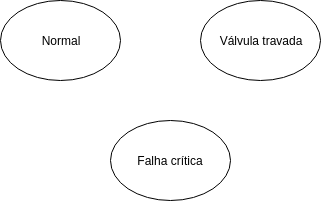
\includegraphics[width=\textwidth,height=\textheight,keepaspectratio]{figuras/_grafo_yuri_no_edge.png}
        	    \caption{Estados do processo}
        	    \label{fig:estados}
        	\end{figure}
    \end{columns}
\end{frame}


\begin{frame}{Objetivos}
    \begin{columns}
        \column{.4\textwidth}
        	\begin{itemize}
        	    \item Detectar modos de operação de não supervisionada
        	    \item Detectar relações entre modos de operação
        	    \item Validar com dados provenientes de sistemas reais
        	\end{itemize}
    	
    	\column{.6\textwidth}
        	\begin{figure}
        	    \centering
        	    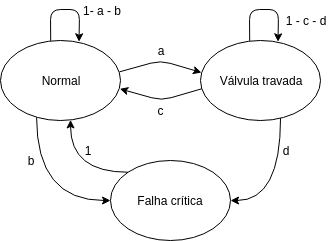
\includegraphics[width=\textwidth,height=\textheight,keepaspectratio]{figuras/grafo_yuri.png}
        	    \caption{Modelo Evolutivo}
        	    \label{fig:grafo}
        	\end{figure}
    \end{columns}
\end{frame}


\begin{frame}{Objetivos}
    \begin{columns}
        \column{.4\textwidth}
        	\begin{itemize}
        	    \item Detectar modos de operação de não supervisionada
        	    \item Detectar relações entre modos de operação
        	    \item Validar com dados provenientes de sistemas reais
        	\end{itemize}
    	
    	\column{.6\textwidth}
        	\begin{figure}
        	    \centering
        	    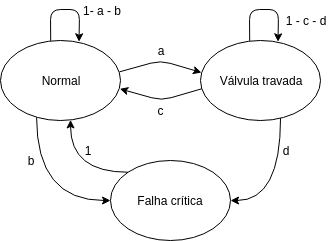
\includegraphics[height=.18\textheight,keepaspectratio]{figuras/grafo_yuri.png}
        	    \caption{Modelo evolutivo}
        	    \label{fig:grafo_industria}
        	\end{figure}
        	\begin{figure}
        	    \centering
        	    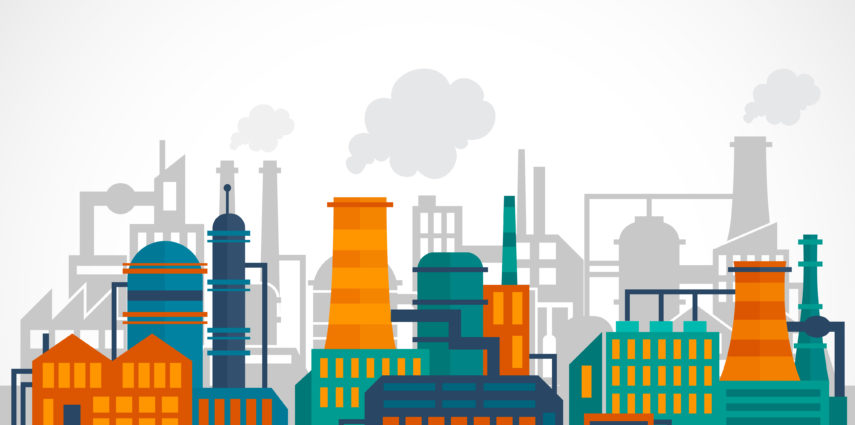
\includegraphics[height=.18\textheight,keepaspectratio]{figuras/industria.jpg}
        	    \caption{Indútria}
        	    \label{fig:industria}
        	\end{figure}
    \end{columns}
\end{frame}

% Aplicações
\section{Aplicações}
\begin{frame}{Aplicações}
    \begin{itemize}
        \item Seleção de contexto de dados para monitoramento de alarmes: Baseado no estado e nos possíveis estados acessíveis selecionar os conjuntos de alarme que devem ter maior prioridade para os operadores.
        \item Predição de operação: Estimar produção, prever paradas, planejamento de manunteção.
        \item Análise de causa raiz: Após a ocorrência de uma anormalidade é possível revisitar os estados pelos quais o processo transitou a partir da normalidade e analisar os primeiros estágios anormais do processo facilitando a detecção da causa raiz. 
    \end{itemize}
\end{frame}

% Conclusão
\section{Conclusão}

% Cronograma
\begin{frame}{Cronograma}
    \begin{table}[]
        \begin{tabular}{l|l|l|l|l|l|l|l|l|}
            \cline{2-9}
                                                          & \multicolumn{2}{l|}{2019} & \multicolumn{2}{l|}{2020} & \multicolumn{2}{l|}{2021} & \multicolumn{2}{l|}{2022} \\ \cline{2-9} 
                                                          & 1º          & 2º          & 1º          & 2º          & 1º          & 2º          & 1º          & 2º          \\ \hline
            \multicolumn{1}{|l|}{Disciplinas}             & X           & X           & X           &             &             &             &             &             \\ \hline
            \multicolumn{1}{|l|}{Revisão bibliográfica}   & X           & X           &             &             &             &             &             &             \\ \hline
            \multicolumn{1}{|l|}{Redação da Qualificação} &             &             & X           & X           &             &             &             &             \\ \hline
            \multicolumn{1}{|l|}{Qualificação}            &             &             &             & X           &             &             &             &             \\ \hline
            \multicolumn{1}{|l|}{Redação da Tese}         &             &             &             &             & X           & X           & X           & X           \\ \hline
            \multicolumn{1}{|l|}{Defesa da Tese}          &             &             &             &             &             &             &             & X           \\ \hline
            \multicolumn{1}{|l|}{Produção de Artigo}      &             &             & X           &             & X           &             & X           &             \\ \hline
        \end{tabular}
    \end{table}
\end{frame}

% Resumo
\begin{frame}{Resumo}
    \begin{columns}
	    \column{.5\textwidth}

	    \column{.5\textwidth}

	\end{columns}
\end{frame}

% Referências
% \begin{frame}{References}
%     \printbibliography
% \end{frame}
% \begin{frame}{References}
%     \printbibliography
% \end{frame}

\begin{frame}[allowframebreaks]{References}
\printbibliography
\end{frame}


\end{document}